\section{Otimização e Engenharia de Reservatório}
\subsection{Contexto}
Na engenharia de reservatórios, os pesquisadores buscam métodos visando à melhoria das condições e resultados produtivos dos reservatórios existentes. Atualmente, estima-se que até 60\% de óleo podem ser recuperados a partir do emprego de técnicas de EOR \footnote{Informação disponível em <http://energy.gov/fe/science-innovation/oil-gas-research/enhanced-oil-recovery>. Acesso em: 17 de Setembro de 2018}. De acordo com Udy \textit{et al.}, métodos de EOR e de injeção de água são utilizados, a depender das propriedades e do estado de produção do reservatório, de maneira a se encontrar condições ótimas de produção de óleo ou de NPV \cite{udyEOR}.

Geralmente, os engenheiros de reservatório e de produção buscam encontrar alocações de recursos de produção por meio de simulações computacionais baseadas na estratégia de tentativa e erro; contudo, tal abordagem reduz a probabilidade de se encontrar as condições ótimas de produção, uma vez que poucos cenários são considerados. Além disso, como é inviável a obtenção de uma grande quantidade de simulações, os resultados conduzem a condições não otimizadas e redução da produção total. Além das limitações computacionais, outros desafios se tornam presentes na otimização da produção de petróleo, a saber: a falta de dados históricos adequados para a calibração do modelo matemático, as discrepâncias presentes nos parâmetros físicos, a imprevisibilidade dos preços do óleo e do gás, entre outros\footnote{Ver \cite{udyEOR}}.

No esforço de se encontrar as melhores condições de operação de reservatórios, foram feitas tentativas de se desenvolver simuladores que conseguissem obter os melhores esquemas de produção, combinando simulações de reservatório com algoritmos de busca linear; entretanto, simuladores baseados em diferenças finitas possuem uma multitude de variáveis e relações que não se integram facilmente aos métodos numéricos de otimização. A chave para o método proposto é se obter uma diferenciação total do simulador, assim tornando-se possível a computação eficiente e precisa de buscas de gradiente direcional \cite{asheim88}. 

No campo da engenharia de reservatório, são utilizados tanto algoritmos de gradiente descendente quanto meta-heurísticos na resolução de problemas de otimização. Serão analisadas duas classes de problemas envolvendo reservatórios: maximização da produção de óleo e do NPV, e posicionamento de poços.
\nocite{EOR:Intro}


\subsection{Algoritmos de Gradiente Descendente}
O uso de algoritmos de gradiente descendente está bastante difundido na engenharia de reservatórios, em particular em situações em que se busca otimizar a produção e o NPV. Fonseca \textit{et al.}, por exemplo, utiliza variações estocásticas do algoritmo simplex, de maneira a se lidar com as incertezas de simulação e, assim, buscar o resultado ótimo, comparando a solução proposta com algoritmos de otimização robusta \cite{fonseca}; Asheim descreve um algoritmo utilizando busca linear em conjunto com as condições KKT, calculando sucessivamente o NPV durante o algoritmo, ilustrado pela Figura \ref{fig:asheim1} \cite{asheim88}.

\begin{figure}[H]
	\centering
	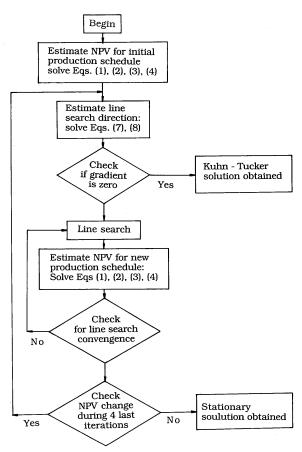
\includegraphics[width=.5\textwidth]{figs/revisao/revisao_asheim1}
	\caption{Exemplo de algoritmo de gradiente descendente aplicado para NPV \cite{asheim88}\label{fig:asheim1}}
\end{figure}

Os algoritmos envolvendo gradientes podem também ser acrescidos de métodos adjuntos; Essen \textit{et al.}, por exemplo, usam esses métodos em conjunto com um algoritmo de otimização robusta aplicado a um conjunto de 100 realizações de um reservatório\footnote{Ver \cite{SPE:RWO}.}, enquanto que Liu e Reynolds utilizam um NBI (\textit{Normal Boundary Intersection}) com uso de uma função Lagrangiana aumentada, em que os gradientes necessários são computados por métodos adjuntos \cite{GEO:LIU}; nesse último caso, dois problemas envolvendo injeção de água foram considerados: o primeiro problema almejava maximizar o NPV da vida útil do reservatório e o NPV a curto prazo; já o segundo problema, aplicado a uma descrição incerta de um reservatório, tinha como objetivo maximizar o valor esperado do NPV durante o ciclo de produção do reservatório e diminuir o desvio padrão do NPV em um conjunto de realizações geológicas\footnote{Ver \cite{GEO:LIU}.}.

Outros algoritmos considerados de gradiente descendente, além dos já descritos, são utilizados também em problemas envolvendo injeção de água; Asadollahi e N{\ae}vdal, por exemplo, utilizam uma combinação do método da descida rápida com o gradiente conjugado com vistas à maximização da produção. A solução obtida é então testada em outras realizações do mesmo reservatório, obtidas por meio de ajuste de histórico, de maneira a se testar a robustez da mesma \footnote{Ver \cite{SPE:WFO}.}. Além dos métodos já citados, outro algoritmo presente na literatura é o SQP: Grema \textit{et al.} utilizam o SQP em um reservatório cujo modelo, resultante de uma identificação, é uma rede neural do tipo NARX (\textit{Nonlinear Autoregressive with Exogenous Input})\footnote{O modelo NARX pode ser encontrado em \cite[p. 390]{aguirre}.}; a simulação foi conduzida com uso do MRST \cite{grema2017optimization}. Já Lorentzen \textit{et al.} usam o SQP em conjunto com um Filtro de Kalman especial, denominado \textit{Ensemble Kalman Filter} --- o filtro é utilizado durante a assimilação dos dados, e o SQP é destinado à obtenção do NPV ótimo, sendo o número de variáveis do problema inicialmente reduzido \cite{lorentzen2009sqp}.

Os problemas envolvendo posicionamento de poços, ao contrário da otimização por meio do NPV, possuem menor número de publicações em que são utilizados métodos envolvendo gradientes; Sarma e Chen explicam esse fato partindo da premissa que as posições dos poços são discretas, e que o gradiente da função objetivo em respeito a esses parâmetros não é definido; contudo, os mesmos autores descrevem uma adaptação do problema em que a função de posicionamento dos poços é adaptada para um modelo contínuo, possibilitando o uso de algoritmos de gradiente descendente. Ainda assim, eles destacam que, em problemas de posicionamento de poços, os algoritmos mais utilizados são os meta-heurísticos \cite{sarmaChen}.


\subsection{Algoritmos Meta-heurísticos}
Além dos algoritmos de gradiente descendente, os métodos meta-heurísticos de otimização estão bem difundidos na literatura, no que diz respeito à resolução tanto de problemas de obtenção de condições ótimas de produção quanto de posicionamento inteligente de poços. Entre os algoritmos utilizados, destacam-se os algoritmos genéticos (GA), o PSO, o \textit{simulated annealing} (SA), entre outros.

Em problemas de otimização da produção, notadamente em esquemas de explotação envolvendo o uso da injeção de água, os algoritmos genéticos têm destaque: Mamghaderi e Pourafshary buscam maximizar a produção de óleo alocando volumes de água nos injetores, utilizando um algoritmo genético em conjunção com um modelo capacitor-resistor (CRM)\footnote{O CRM é explicado e utilizado em \cite{SAYARPOUR2009227}.} \cite{MAMGHADERI2013107}; 
